
\section{System Architecture Overview}
The system is composed of four tightly integrated layers: (1) a CNN-based pose classifier, (2) a MediaPipe skeletal landmark engine, (3) a biomechanical pose rules engine, and (4) a voice-driven coaching loop. Figure~\ref{fig:architecture} illustrates the high-level data flow.

\begin{figure}[H]
    \centering
    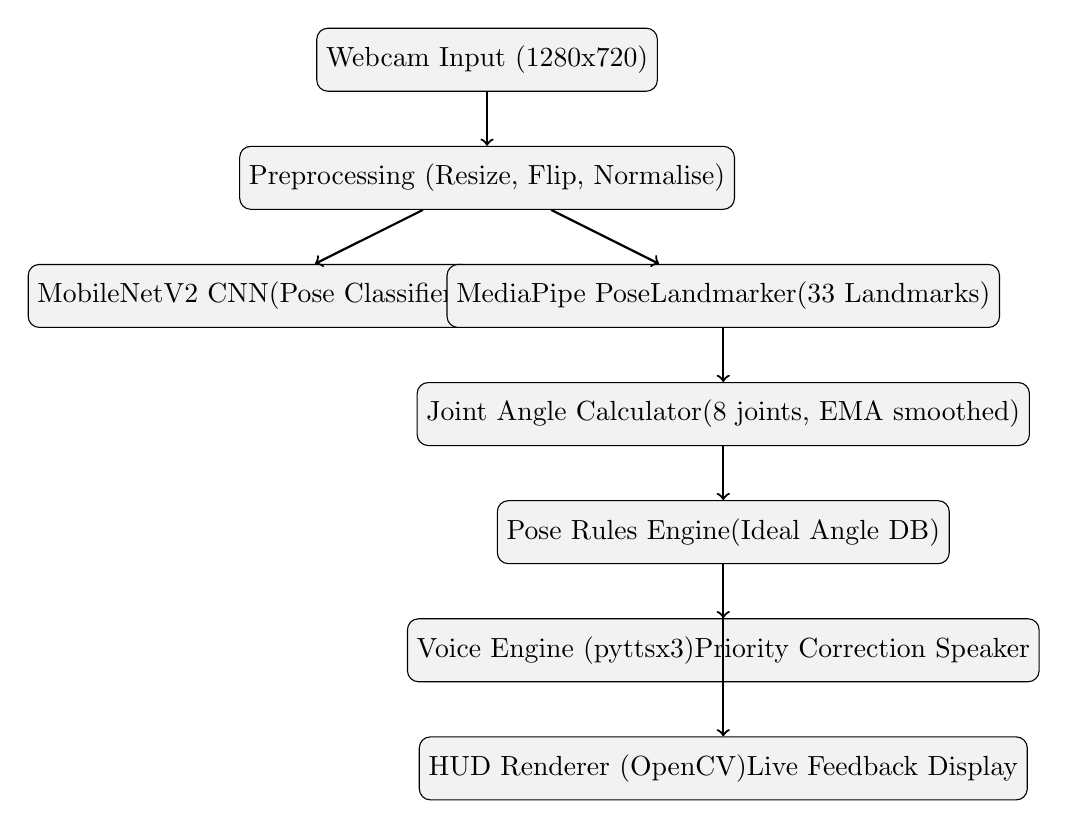
\begin{tikzpicture}[
        node distance = 1.5cm,
        box/.style={rectangle, draw, rounded corners, minimum width=4cm, minimum height=0.8cm, text centered, fill=gray!10},
        arrow/.style={->, thick}
    ]
        \node[box] (cam) {Webcam Input (1280x720)};
        \node[box, below of=cam] (preproc) {Preprocessing (Resize, Flip, Normalise)};
        \node[box, below of=preproc, xshift=-3cm] (cnn) {MobileNetV2 CNN \\ (Pose Classifier)};
        \node[box, below of=preproc, xshift=3cm] (mp) {MediaPipe PoseLandmarker \\ (33 Landmarks)};
        \node[box, below of=mp] (angle) {Joint Angle Calculator \\ (8 joints, EMA smoothed)};
        \node[box, below of=angle] (rules) {Pose Rules Engine \\ (Ideal Angle DB)};
        \node[box, below of=rules] (voice) {Voice Engine (pyttsx3) \\ Priority Correction Speaker};
        \node[box, below of=voice] (hud) {HUD Renderer (OpenCV) \\ Live Feedback Display};

        \draw[arrow] (cam) -- (preproc);
        \draw[arrow] (preproc) -- (cnn);
        \draw[arrow] (preproc) -- (mp);
        \draw[arrow] (mp) -- (angle);
        \draw[arrow] (angle) -- (rules);
        \draw[arrow] (rules) -- (voice);
        \draw[arrow] (rules) -- (hud);
    \end{tikzpicture}
    \caption{High-Level System Architecture}
    \label{fig:architecture}
\end{figure}

\section{Main Application Loop Flowchart}
The core operational logic of the application (\texttt{app.py}) follows a continuous loop that integrates vision, inference, and feedback. Figure~\ref{fig:main_loop} provides a detailed view of the per-frame processing cycle.

\begin{figure}[H]
    \centering
    \begin{tikzpicture}[
        node distance = 1.3cm,
        start/.style={ellipse, draw, fill=green!10, minimum width=2.5cm},
        decision/.style={diamond, draw, fill=yellow!10, aspect=2, text centered, inner sep=0pt},
        process/.style={rectangle, draw, fill=blue!5, minimum width=3.5cm, minimum height=0.8cm},
        arrow/.style={->, thick}
    ]
        \node[start] (start) {Start Loop};
        \node[process, below of=start] (cap) {Capture Frame};
        \node[process, below of=cap] (prep) {Preprocess \& Resize};
        \node[process, below of=prep] (cnn) {Run CNN Classifier};
        \node[process, below of=cnn] (buffer) {Buffer Predictions};
        \node[process, below of=buffer] (mp) {Run MediaPipe Detection};
        \node[decision, below of=mp, yshift=-0.5cm] (vis) {Body Visible?};
        \node[process, right of=vis, xshift=3.5cm] (warn) {Issue Visibility Warning};
        \node[process, below of=vis, yshift=-1cm] (calc) {Calc Smoothed Angles};
        \node[process, below of=calc] (fsm) {Update FSM State};
        \node[process, below of=fsm] (rules) {Evaluate Pose Rules};
        \node[process, below of=rules] (hud) {Render HUD Overlay};
        \node[process, below of=hud] (show) {Display Frame};
        
        \draw[arrow] (start) -- (cap);
        \draw[arrow] (cap) -- (prep);
        \draw[arrow] (prep) -- (cnn);
        \draw[arrow] (cnn) -- (buffer);
        \draw[arrow] (buffer) -- (mp);
        \draw[arrow] (mp) -- (vis);
        \draw[arrow] (vis) -- node[above] {No} (warn);
        \draw[arrow] (vis) -- node[left] {Yes} (calc);
        \draw[arrow] (warn) |- (hud);
        \draw[arrow] (calc) -- (fsm);
        \draw[arrow] (fsm) -- (rules);
        \draw[arrow] (rules) -- (hud);
        \draw[arrow] (hud) -- (show);
        \draw[arrow] (show) -- ++(-4,0) |- (cap);
    \end{tikzpicture}
    \caption{Detailed Main Application Loop Flowchart}
    \label{fig:main_loop}
\end{figure}

\section{CNN Model Design — MobileNetV2 Transfer Learning}
\subsection{Architecture Details}
The pose classifier is built using MobileNetV2 pre-trained on ImageNet as a feature extractor. The top classification head is replaced with a custom stack tailored for five-class yoga classification.

The Base Model utilizes MobileNetV2 with an input shape of 224$\times$224$\times$3, excluding the top classification layer. The backbone outputs a 7$\times$7$\times$1280 feature map, which contains rich spatial information about the pose silhouette.

A Global Average Pooling layer is then applied to reduce the spatial dimensions, resulting in a 1280-dimensional feature vector that summarizes the entire image. This is followed by a Dropout layer with a rate of 0.5 to prevent overfitting on the relatively small yoga dataset.

A Dense Layer with 256 units and ReLU activation provides the non-linear capacity to discriminate between the specific yoga poses. L2 regularization with a coefficient of $10^{-4}$ is applied to the weights of this layer to maintain model simplicity and generalization.

A Batch Normalization layer follows the dense layer to stabilize the activations and accelerate the training process. An additional Dropout layer with a rate of 0.3 is applied for further regularization. Finally, the Output Layer consists of a 5-unit Softmax activation, producing the probability scores for each of the five yoga classes.

\subsection{Two-Stage Training Strategy}
Training proceeds in two stages to optimize the transfer learning process.

In Stage 1 (Feature Extraction), the MobileNetV2 backbone is frozen, meaning its weights are not updated. Only the custom classification head is trained for 10 epochs using the Adam optimizer with a learning rate of $10^{-3}$. This allows the head to learn to interpret the pre-trained features before the backbone itself is modified.

In Stage 2 (Fine-Tuning), the last 54 layers of the backbone (layers from index 100 onward) are unfrozen. This allows the network to adapt its higher-level feature representations to the specific characteristics of yoga imagery, such as limbs and body alignments. Training resumes for 25 additional epochs with a significantly reduced learning rate of $10^{-5}$ to prevent the weights from diverging too far from the optimal ImageNet-trained state.

\subsection{Training Callbacks}
The training process is monitored and managed by several Keras callbacks. The \texttt{ModelCheckpoint} callback ensures that only the version of the model with the best validation accuracy is saved. The \texttt{ReduceLROnPlateau} callback automatically halves the learning rate if the validation loss stagnates for 3 epochs, helping the model converge to a flatter minimum. Finally, the \texttt{EarlyStopping} callback terminates the training if validation loss does not improve for 7 consecutive epochs, saving time and preventing overfitting.

\section{MediaPipe Landmark Extraction and Smoothing}
The \texttt{PoseEstimator} class wraps the MediaPipe Tasks API \texttt{PoseLandmarker} (Lite variant) to handle skeletal tracking.

The processing pipeline begins by accepting a BGR frame from OpenCV, converting it to RGB, and wrapping it in a \texttt{mediapipe.Image} object. The landmarker's \texttt{detect()} method is then called to produce 33 normalized 3D body landmarks. These coordinates are converted from normalized $[0,1]$ space to pixel coordinates by scaling them by the frame's dimensions.

To address the inherent jitter in real-time landmark detection, an Exponential Moving Average (EMA) smoothing filter is applied. The filter follows the formula $\hat{x}_t = \alpha \cdot x_t + (1 - \alpha) \cdot \hat{x}_{t-1}$, with a smoothing factor $\alpha$ set to $0.10$. This approach ensures that 90\% of the previous frame's position is retained, effectively suppressing high-frequency noise while still allowing the system to track user movements with acceptable latency.

\section{Joint Angle Calculation}
For each of eight joints, including the left and right shoulders, elbows, hips, and knees, three landmark indices $(A, B, C)$ are defined, where $B$ represents the joint vertex. The angle at $B$ is computed using the vector representation of the limbs: $\theta = \left| \arctan2\left(\vec{BC}_y, \vec{BC}_x\right) - \arctan2\left(\vec{BA}_y, \vec{BA}_x\right) \right|$. The resulting angle in radians is converted to degrees and mapped to the range $[0°, 180°]$. This mapping simplifies the rule-based comparison by providing a standard anatomical angle.

\section{Pose Rules Engine and Scoring}
The \texttt{pose\_rules.py} module manages the hand-crafted ideal angle database for the target poses. Each rule entry specifies the minimum and maximum ideal angles, along with confirmation and corrective messages.

The scoring function evaluates the measured angles against these rules with a global tolerance of $\pm 15$ degrees. If an angle falls within the specified range, the joint is marked as correct. The system returns a collection of correction objects and calculates an overall correctness score as the percentage of joints that meet their respective criteria.

\section{Finite State Machine (FSM) Design}
The application's guided training session is governed by a five-state Finite State Machine, as illustrated in Figure~\ref{fig:fsm_diagram}.

\begin{figure}[H]
    \centering
    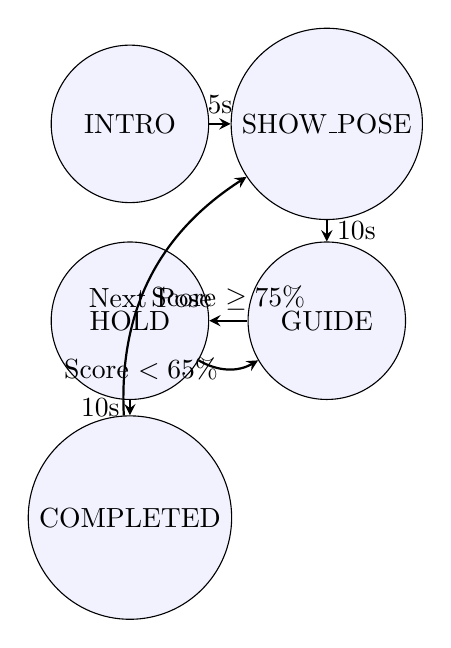
\begin{tikzpicture}[
        node distance = 2.5cm,
        state/.style={circle, draw, minimum size=2cm, text centered, fill=blue!5},
        arrow/.style={->, thick, >=stealth}
    ]
        \node[state] (intro) {INTRO};
        \node[state, right of=intro] (show) {SHOW\_POSE};
        \node[state, below of=show] (guide) {GUIDE};
        \node[state, left of=guide] (hold) {HOLD};
        \node[state, below of=hold] (comp) {COMPLETED};

        \draw[arrow] (intro) -- node[above] {5s} (show);
        \draw[arrow] (show) -- node[right] {10s} (guide);
        \draw[arrow] (guide) -- node[above] {Score $\geq 75\%$} (hold);
        \draw[arrow] (hold) edge[bend right] node[left] {Score $< 65\%$} (guide);
        \draw[arrow] (hold) -- node[left] {10s} (comp);
        \draw[arrow] (comp) edge[bend left] node[below] {Next Pose} (show);
    \end{tikzpicture}
    \caption{Finite State Machine for Yoga Training Routine}
    \label{fig:fsm_diagram}
\end{figure}

The \textbf{INTRO} state welcomes the user and provides a brief preparation period. In the \textbf{SHOW\_POSE} state, the system displays a reference image of the target pose and prepares the user for instruction. The \textbf{GUIDE} state is the core active phase, where real-time skeletal overlays and priority-ranked voice corrections are provided. Once the user achieves a correctness score of $\geq 75\%$, the system transitions to the \textbf{HOLD} state, where a 10-second countdown begins. If the score falls below a safety threshold of 65\%, the system reverts to the GUIDE state. Upon successful completion of the hold duration, the state transitions to \textbf{COMPLETED}, and the routine advances to the next pose.

\section{Voice Engine and Priority Mechanism}
The \texttt{VoiceEngine} class utilizes the \texttt{pyttsx3} library running in a dedicated background thread to ensure non-blocking audio output. To prevent constant chatter, a minimum interval of 4 seconds is enforced between successive spoken corrections.

The system employs a priority mechanism that ranks all incorrect joints based on the magnitude of their deviation from the ideal midpoint of their target range. Only the single most critical correction is spoken during any given interval. This approach allows the user to focus on significant form errors one by one, mimicking the behavior of a professional instructor who prioritizes critical adjustments over minor ones.

\section{Visual HUD Design and User Feedback}
The real-time Heads-Up Display (HUD) provides a comprehensive visual feedback system for the practitioner.

The Header Bar at the top of the frame displays the application title, the current target pose name, and the cumulative correctness score as a percentage. A dynamic Timer and State Indicator provide real-time updates on the progress of the current training phase.

The Skeleton Overlay is rendered directly on the user's video feed, with white lines representing the bones and color-coded rings at each joint. Joints that are correctly aligned according to the rules engine are marked in green, while those requiring adjustment are highlighted in red. Angle Labels, including magenta arc indicators and degree values, provide specific quantitative feedback at each joint.

A Footer Bar provides a rolling list of all active textual corrections, allowing the user to see exactly what needs to be changed. Additionally, a Picture-in-Picture inset displays a reference image of the target pose, providing a constant visual guide for the user to emulate.
